\section*{DATA}\label{data}}
The data used in this study is described in
Tab.\ref{tab:data_files}. There is one result with a pure FNPF
simulation at 0 knots. For model test results, two tests are available
at 0 knots and one test at 15.5 knots. There is also a result at 15.5
with a hybrid method, where semi empirical viscosity has been injected
into the FNPF calculations.
\begin{table}[H]
\scriptsize
\center
\caption{Data files}
\label{tab:data_files}
\begin{tabular}{|l|l|l|l|}
\hline\addlinespace
file & data file & Ship speed & Method\\
&  & $[kts]$ & \\
\hline1 & \text{fnpf_kvlcc2_rolldecay_0kn.csv} & 0.0 & FNPF\\
2 & \text{model_test_21337.csv} & 0.0 & model test\\
3 & \text{model_test_21338.csv} & 0.0 & model test\\
4 & \text{model_test_21340.csv} & 15.5 & model test\\
5 & \text{fnpf_kvlcc2_rolldecay_15-5kn_ikeda_dev.csv} & 15.5 & hybrid\\
\hline
\end{tabular}
\end{table}
Fig. \ref{fig:all_tests} shows the roll angle time series for
all the tests. It can also be seen that test 1 and 5 also have time
series for the roll angle velocity and acceleration from the conducted
FNPF simulations. For the model test (2,3,4) velocities and
accelerations were not measured during the tests.
\begin{figure}[H]
\begin{center}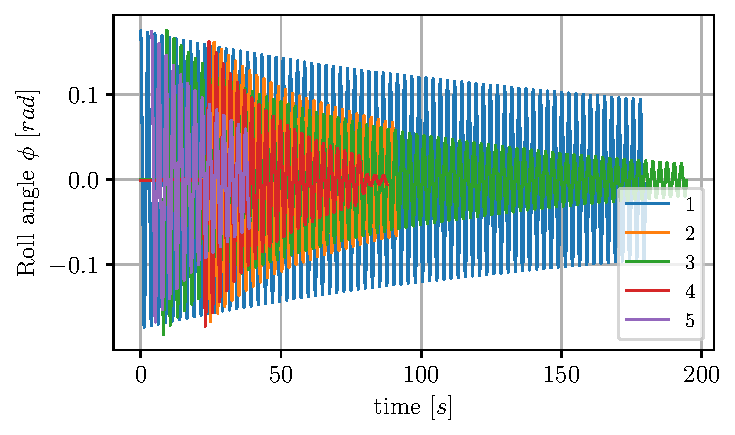
\includegraphics[width = 0.95\textwidth]{figures/all_tests.pdf}\end{center}
\vspace{-0.7cm}
\caption{All tests}
\label{fig:all_tests}
\end{figure}
\begin{figure}[H]
\begin{center}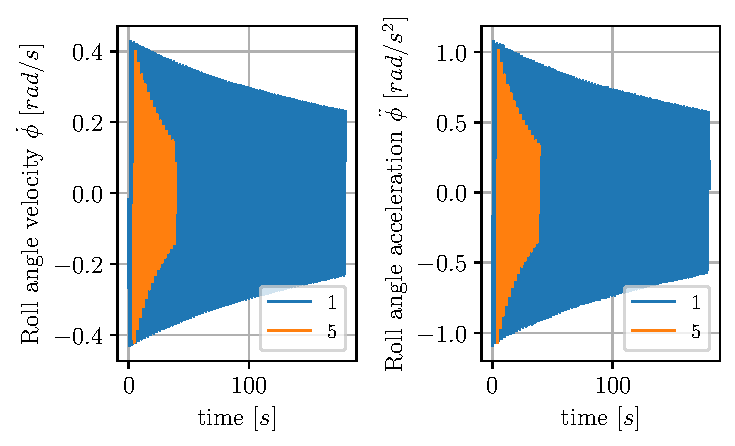
\includegraphics[width = 0.95\textwidth]{figures/vel_acc.pdf}\end{center}
\vspace{-0.7cm}
\caption{Tests with velocities and accelerations}
\label{fig:vel_acc}
\end{figure}
\hypertarget{analysis}{%
